\chapter{Data, Trigger and Event Selection}

\section{Introduction}

\section{Data}

CMS started taking collisions in date at $\sqrt{s} = 900 \GeV$. The centre of
mass energy was increased to 1.37 TeV representing a new record in centre of
mass energy at a collider. Since March 2011 CMS has been taking 7 TeV 
collisions data. 7 TeV is the centre of mass energy of the data used in this 
thesis. \\

The higher centre of mass energy increases the production cross-section of
certain processes, in particular stong production SUSY, and also enables the
production of more massive particles. It should be noted that the important
energy is not the centre of mass energy of the proton collision, but that of the
parton collision. Since there are 6 partons in each proton, 3 quarks and 3
gluons, the centre of mass energy of the average parton collision is about 1.2
TeV. So CMS is sensitive to TeV scale physics. \\   

The luminosity has also increased over time. As the integrated luminosity 
increases more statistics are available to improve the significance of 
observations and the accuracy of measurements. There are two ways to increase 
the luminosity: increase the intensity of the beams and increase the number of
bunches. Both have been done in the LHC. Increasing the luminosity leads to
more interactions per bunch crossing -- an effect called pile-up. During 2011
data taking the luminosity has increased from x to y. \\

Figure \ref{fig:intlumi} shows the integrated luminosity recorded by CMS over 
time until September 2011. \\

\begin{figure}
\begin{center}
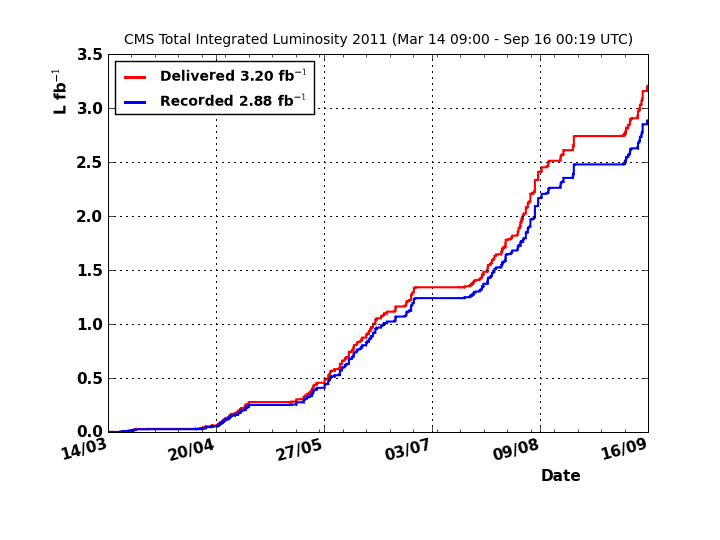
\includegraphics[width=0.8\textwidth]{Integrated_Luminosity.png}
\caption{The integrated luminosity vs time delivered to (red) and recorded by
(blue) CMS during stable beams at $\sqrt{s} = 7 \TeV$.}
\end{center}
\label{fig:intlumi}
\end{figure}

The data used for this analysis is the EPS data set containing $1.1 \invfb$
at $\sqrt{s} = 7 \TeV$ taken from March to June 2011. This corresponds to the
run range 160404 to 171106. Only data certified by the physics validation team
is included in the data set. The data sets used in this analysis are listed 
below.

\begin{itemize}
\item /PhotonHad/Run2011A-May10ReReco-v1/AOD %(Run 160404 - 163817) 
\item /PhotonHad/Run2011A-PromptReco-v4/AOD %(Run 165071 - 168437)
\item /PhotonHad/Run2011A-PromptReco-v5/AOD %(Run 170053 - 171106)
\end{itemize} \\

The data is split into Primary Datasets each with different trigger
requirements. PhotonHad is one such Primary Dataset. \\

Re-processing of the data is performed periodically to ensure that data
reconstructed using a much older version of the software is not analysed
together with the most recent data reconstructed with the latest software
version. The May10ReReco above is one such re-processing. The software version
used to reconstruct the data is CMSSW\_4\_2\_3\_patch2. CMSSW being the standard
CMS reconstruction software. The reconstruction involves building jets, 
electrons, photons and other physics objects form the raw energy deposits in the
detector.

\section{Monte Carlo Samples}

Since the background estimation (see \ref{sec:}) is largely data-driven the
dependence of the result on the MC samples is limited. The QCD background
estimation is entirely data driven and the QCD MC is used only for the error on
the background estimation. MC samples are used to estimate EWK and ttbar
backgrounds, but these are insignificant compared to the QCD background. \\

The Monte Carlo samples used in this analysis are listed below. \\

{\bf QCD}

/QCD\_Pt-50to80\_TuneZ2\_7TeV\_pythia6/Summer11-PU\_S4\_START42\_V11-v1/AODSIM
/QCD\_Pt-80to120\_TuneZ2\_7TeV\_pythia6/Summer11-PU\_S4\_START42\_V11-v1/AODSIM
/QCD\_Pt-120to170\_TuneZ2\_7TeV\_pythia6/Summer11-PU\_S4\_START42\_V11-v1/AODSIM
/QCD\_Pt-170to300\_TuneZ2\_7TeV\_pythia6/Summer11-PU\_S4\_START42\_V11-v1/AODSIM
/QCD\_Pt-300to470\_TuneZ2\_7TeV\_pythia6/Summer11-PU\_S4\_START42\_V11-v1/AODSIM
/QCD\_Pt-470to600\_TuneZ2\_7TeV\_pythia6/Summer11-PU\_S4\_START42\_V11-v1/AODSIM
/QCD\_Pt-600to800\_TuneZ2\_7TeV\_pythia6/Summer11-PU\_S4\_START42\_V11-v1/AODSIM
/QCD\_Pt-800to1000\_TuneZ2\_7TeV\_pythia6/Summer11-PU\_S4\_START42\_V11-v1/AODSIM
/QCD\_Pt-1000to1400\_TuneZ2\_7TeV\_pythia6/Summer11-PU\_S4\_START42\_V11-v1/AODSIM
/QCD\_Pt-1400to1800\_TuneZ2\_7TeV\_pythia6/Summer11-PU\_S4\_START42\_V11-v1/AODSIM
/QCD\_Pt-1800\_TuneZ2\_7TeV\_pythia6/Summer11-PU\_S4\_START42\_V11-v1/AODSIM \\

/G\_Pt-50to80\_TuneZ2\_7TeV\_pythia6/Summer11-PU\_S4\_START42\_V11-v1/AODSIM
/G\_Pt-80to120\_TuneZ2\_7TeV\_pythia6/Summer11-PU\_S4\_START42\_V11-v1/AODSIM
/G\_Pt-120to170\_TuneZ2\_7TeV\_pythia6/Summer11-PU\_S4\_START42\_V11-v1/AODSIM
/G\_Pt-170to300\_TuneZ2\_7TeV\_pythia6/Summer11-PU\_S4\_START42\_V11-v1/AODSIM
/G\_Pt-300to470\_TuneZ2\_7TeV\_pythia6/Summer11-PU\_S4\_START42\_V11-v1/AODSIM
/G\_Pt-470to800\_TuneZ2\_7TeV\_pythia6/Summer11-PU\_S4\_START42\_V11-v1/AODSIM \\

{\bf EWK}

/WToENu\_TuneZ2\_7TeV-pythia6/Summer11-PU\_S3\_START42\_V11-v2/AODSIM
/ZGToNuNuG\_TuneZ2\_7TeV-madgraph/Summer11-PU\_S4\_START42\_V11-v1/AODSIM \\

{\bf ttbar}

/TTJets\_TuneZ2\_7TeV-madgraph-tauola/Summer11-PU\_S4\_START42\_V11-v1/AODSIM \\

The Monte Carlo samples are generated using Pythia 6 \cite{pythia6} or Madgraph
\cite{madgraph} with Tune Z2 (based on CTECQ6 parton distribution functions 
\cite{tuneZ2}). GEANT \cite{geant}is used for the detector simulation. \\

Pile-up is simulated in all Monte Carlo samples however the MC does not
reproduce the nVertices distribution seen in the data. reweighting.

\section{Trigger}

As the luminosity has increased more stringent trigger requirements have been 
necessary to keep the data rate manageable. 

\section{Photon Selection}

Fake photons from QCD come from jets and so tend to have plenty of activity in
the surrounding detectors. In contrast, prompt photons tend to be isolated with
little surrounding activity. Isolation is one of the variables used to select 
photons because of its background rejection power. There are three independent 
isolation measures based on the ECAL, the HCAL and the tracker. \\

Fake photons from jets also tend to have a hadronic component as well as an
electromagnetic component while prompt photons are purely electromagnetic. \\ 

Photons are detected by an electromagnetic shower in the ECAL. Prompt photons
can be distinguished from fakes by the shower shape. \\

Photons are distinguished from electrons by the tracker. Electrons, being
charged particles, ionise in the silicon tracker and so leave a track. Photons
do not. \\ 

Based on these considerations, there are six variables used for the photon 
selection:

\begin{itemize}
\item ECAL isolation
\item HCAL isolation
\item Track isolation
\item H/E
\item Shower Shape ($\sigma_{i\eta i\eta}$)
\item Pixel Seed
\end{itemize}

ECAL isolation is defined as the sum of the energy deposited in the crystals of 
the ECAL in a $\Delta R = 0.4$ circle around the photon. A smaller circle of 
$\Delta R = 0.1$ around the photon is excluded from the isolation sum to avoid 
counting the photon itself in the isolation. Also a strip along $\phi$ of width 
$\Delta \eta = 0.04$ is excluded from the isolation sum to avoid including 
bremstrahlung from electrons. \\

HCAL isolation is defined as the sum of the energy deposited in the HCAL towers
in a $\Delta R = 0.4$ circle around the photon position. A smaller circle of 
$\Delta R = 0.1$ is excluded from the isolation sum to avoid counting 
rear-leakage from high energy photons in the isolation. \\ 

Track isolation is defined as the sum of the $p_{T}$ of tracks inside a cone of
$\Delta R = 0.4$ around the photon and toward the primary vertex. A hollow cone 
is used $\Delta R < 0.1$ is excluded from the isolation sum. \\

H/E is the ratio of the hadronic energy deposited in the HCAL behind the photon
to the photon energy. Jets faking photons are likely to have a significant 
amount of hadronic energy while for prompt photons the amount of hadronic energy
is likely to be small. \\

The width of the shower in the $\eta$ direction is used as a measure of the
shower shape. The $\eta$ direction rather than the $\phi$ direction is used 
because bremstrahlung can cause electromagnetic showers to be spread out in 
$\phi$. $\sigma_{\eta\eta}$ is the r.m.s width of the shower in the $\eta$ 
direction. The variable used here is $\sigma_{i\eta i\eta}$, which calculates 
the width in terms of number of crystals rather than $\eta$, is better because 
it does not count the gaps between crystals (where there is no showering) in the
width. \\

A pixel seed is a track stub in the pixel detector that is the first step in
track reconstruction. The photon selection requires that there is no pixel seed
corresponding to the electromagnetic shower.

\section{Jet Selection}

\section{Missing Transverse Energy}

\section{Event Selection}

Motivated by SUSY the search is based on missing energy. SUSY events have decay
chains ending in the Lightest Supersymmetric Particle (LSP) which goes
undetected and hence shows up as missing energy. In contrast QCD events, which
are the dominant background, have only fake missing energy due to detector
imperfections (e.g. dead cells). \\

$\HT$, the scalar sum of the transverse momentum of all the objects in the 
event, is used as a measure of the energy scale of the event.

The event selection criteria are listed below. 

\begin{itemize}
\item $\HT > 400 \GeV$
\item $\geq 2$ jets
\item $\geq 1$ photon
\end{itemize}

There is a $\HT$ cut because strongly produced SUSY events have high $\HT$. The 
value of this cut is motivated by the desire for the trigger to be fully 
efficiency for the event selection. \\

The $\geq 2$ jets cut is well motivated from the SUSY perspective: strongly
produced SUSY events start with two squarks/gluinos each of which decay to a 
quark/gluon (which forms a jet in the detector) and the next SUSY particle in 
the mass hierarchy. Parameter points with high gluino mass tend to have only 2 
jets while those with high squark mass tend to have at least 4 jets. \\

In strongly produced Gauge Mediated SUSY Breaking the Next-to-Lightest SUSY 
Particle (NLSP) is the neutralino ($\tilde{\chi}^{0}$) which decays to a photon and 
a gravitino. So at least two photons are expected in each SUSY event. However, 
due to the high activity in these events, photons often fall inside the cone of
a jet and so only one photon is reconstructed. Hence the $\geq 1$ photon cut. \\
